% Relatório da versão 1 do software ipump para o curso
% Sistemas de Controle - DCA0206 - UFRN
% Autores:
%   AUGUSTO MATHEUS PINHEIRO DAMASCENO
%   MARCEL DA CÂMARA RIBEIRO DANTAS
%   PABLO HOLANDA CARDOSO
%   PEDRO DE CASTRO GURGEL LIMA
%   RODRIGO DANTAS DA SILVA
% Modificado por: Ícaro Bezerra Queiroz de Araújo
%

%%%%%%%%%%%% STRUCTURE %%%%%%%%%%%%%%%
\documentclass[a4paper,12pt]{article}
\usepackage[T1]{fontenc}
\usepackage[utf8]{inputenc}
\usepackage[brazil]{babel}
\usepackage{lmodern}
\usepackage{setspace}
\usepackage[top=2cm, bottom=2cm, left=2cm, right=2cm]{geometry}
%%%%%%%%%%%%%%%%%%%%%%%%%%%%%%%%%%%%%%

%%%%%%%%%%%%%%%% PAGES STYLE %%%%%%%%%
\usepackage{fancyhdr}
\fancypagestyle{main}{
\renewcommand{\headrulewidth}{0pt}
\fancyhead[RO]{\thepage}
\fancyfoot[CO]{}
}
%%%%%%%%%%%%%%%%%%%%%%%%%%%%%%%%%%%%%%

\usepackage{graphicx}
\usepackage{float}
\usepackage{epstopdf}
\usepackage{subfig}
\usepackage{mathptmx}
\usepackage{changepage}


\usepackage{listings}
\usepackage{xcolor}
\lstset{language=C++,
                basicstyle=\ttfamily,
                keywordstyle=\color{blue}\ttfamily,
                stringstyle=\color{red}\ttfamily,
                commentstyle=\color{green}\ttfamily,
                morecomment=[l][\color{magenta}]{\#}
}

%\usepackage[alf]{abntex2cite}

%%%%%%%%%%% PDF METADATA %%%%%%%%%%%%%
\usepackage[ pdftitle={MODELO RELATÓRIO},
pdfsubject={INTRODUÇÃO AO LABORATÓRIO DE CONTROLE - Grupo 3},
pdfkeywords={Controle,Automação,UFRN,DCA,ipump},
hidelinks]{hyperref}
%%%%%%%%%%%%%%%%%%%%%%%%%%%%%%%%%%%%%%

\begin{document}

\onehalfspacing

\thispagestyle{empty}

\setcounter{page}{1}

%%%%%%%%%%%% LOGOS %%%%%%%%%%%%%%%%%%%

\begin{figure}[!ht]

\centering

\subfloat{

\includegraphics[width=2.7cm]{UFRN.eps}
\label{UFRN Logo}
}
\hspace{11.09cm}
\subfloat{

\includegraphics[width=2.4cm]{DCA.eps}
\label{DCA Logo}
}

%\caption{}
\label{Logos}

\end{figure}

%%%%%%%%%%%%%%% CAPA %%%%%%%%%%%%%%%%%

\vspace{-1cm}

\begin{center}
{\bf{\normalsize UNIVERSIDADE FEDERAL DO RIO GRANDE DO NORTE\\
CENTRO DE TECNOLOGIA\\
DEPARTAMENTO DE ENGENHARIA DE COMPUTAÇÃO E AUTOMAÇÃO\\
CURSO DE ENGENHARIA DE COMPUTAÇÃO
}}


\vspace{3.6cm}

{\bf{\large RELATÓRIO DA 5ª EXPERIÊNCIA\\
CONTROLE NO ESPAÇO DE ESTADOS: OBSERVADORES DE ESTADO\\
}}
\vspace{1.5cm}
{\large TURMA: 01 A\\
	GRUPO Nº 02}


\vspace{3.6cm}


\begin{flushright}
\begin{normalsize}
ANDRESSA STÉFANY SILVA DE OLIVEIRA: 20160154101\\
\vspace{0.8cm}
FERNANDA MONTEIRO DE ALMEIDA: 20160154228\\
\vspace{0.8cm}
MÁRCIO LUIZ BEZERRA LOPES JÚNIOR: 20160154326\\
\vspace{0.8cm}
VITOR RAMOS GOMES DA SILVA: 20160154415\\
\end{normalsize}
\end{flushright}


\vspace{2.5cm}

{\large Natal-RN\\
2017}

\end{center}

\newpage

%%%%%%%%%%%%%%%  CONTRA-CAPA %%%%%%%%%

\thispagestyle{empty}

\begin{center}
\begin{normalsize}
ANDRESSA STÉFANY SILVA DE OLIVEIRA: 2016015410\\
\vspace{0.8cm}
FERNANDA MONTEIRO DE ALMEIDA 20160154228\\
\vspace{0.8cm}
MÁRCIO LUIZ BEZERRA LOPES JÚNIOR: 20160154326\\
\vspace{0.8cm}
VITOR RAMOS GOMES DA SILVA: 20160154415\\

\end{normalsize}
\end{center}
\vspace{3cm}

{\bf{\large {\centering CONTROLE NO ESPAÇO DE ESTADOS: OBSERVADORES DE ESTADO\\}}}

\vspace{4cm}

\begin{adjustwidth}{7.5cm}{0cm}

{\normalsize
Quinto relatório apresentado à disciplina de
Laboratório de Sistemas de Controle, correspondente à
avaliação da 3º unidade do semestre 2017.1 do 8º período
do curso de Engenharia de Computação da
Universidade Federal do Rio Grande do Norte, sob
orientação do {\bf Prof. Fábio Meneghetti Ugulino de
Araújo} e {\bf Prof. Lucas Costa Pereira Cavalcante.}

}

\end{adjustwidth}

\vspace{2cm}

\begin{center}

Professores:  Fábio Meneghetti Ugulino de Araújo e\\
Lucas Costa Pereira Cavalcante.

\vspace{2.5cm}

{\large Natal-RN\\
2017}

\end{center}

\newpage

%%%%%%%%%%%%%%%  RESUMO %%%%%%%%%%%%%%

\thispagestyle{empty}

\begin{center}
{\large \textbf{RESUMO}}
\end{center}

\vspace{3cm}

\begin{flushleft}

\hspace{4ex}O presente trabalho é a quarta etapa da construção de um aplicativo desktop para controle de sistema de tanques. O software utiliza a comunicação cliente/servidor no qual o sistema de tanques é o servidor. A planta antes utilizada da Quanser foi substituída por uma simulação feita em Java3D, o que eliminou o nível de ruído dos resultados. Nesta etapa do trabalho, o objetivo foi a implementação de controladores P, PI, PD, PID e PI-D de segunda ordem na configuração controle em cascata. A teoria acerca de controle em cascata é introduzida, após é apresentado os resultados dos testes de controle da planta. Por fim, chega-se a conclusão que o controle em cascata tem uma resposta mais rápida em relação às pequenas modificações de nível, mas não tendo a sintonização correta se perde as vantagens adquiridas. \\

\end{flushleft}

\vspace{1.5cm}

\textbf{Palavras-chave:} sistema de tanques; sistema de controle; software; planta Quanser, controlador PID; controle em cascata.

\newpage

%%%%%%%%% LISTA DE FIGURAS %%%%%%%%%%%

\thispagestyle{empty}

\begin{center}
\listoffigures
\end{center}

\newpage

%%%%%%%%%%%%%%% SUMÁRIO %%%%%%%%%%%%%%

\thispagestyle{empty}

\begin{center}
\tableofcontents
\end{center}

\newpage

%%%%%%%%%%%%%%% INTRODUÇÃO %%%%%%%%%%%

\thispagestyle{main}

\section{INTRODUÇÃO}

%\begin{flushleft}
\hspace{4ex}A prática de laboratório 05 tem como objetivo introduzir o conceito de espaço de estados, nesse relatório será apresentado a implementação de um observador de estado para controlar o nível do tanque de baixo da planta \textit{Quanser}, sendo a figura \ref{r2d2e} a representação do simulador da planta:

\begin{figure}[H]
\centering
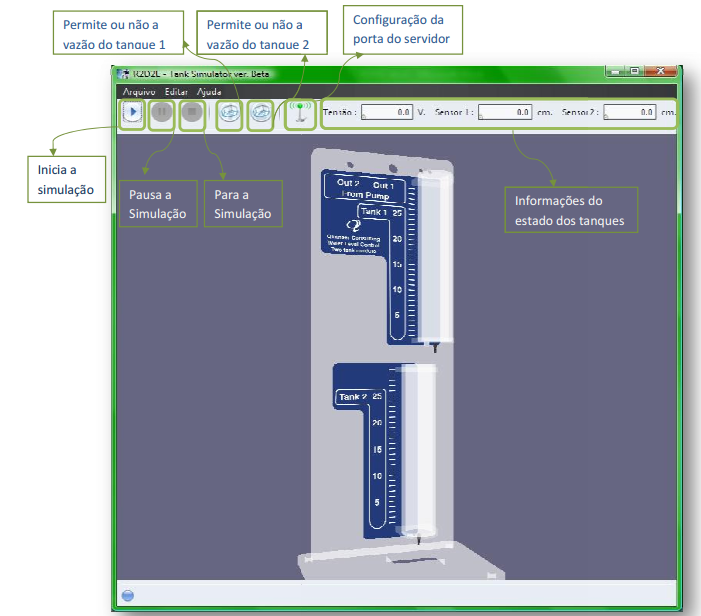
\includegraphics[width=11cm]{ImagensLab4/simulator.png}
\caption{R2D2E - Tank Simulator}
\label{r2d2e}
\end{figure}

\hspace{4ex}Além das opções de controlar os tanques utilizando os controladores Proporcional (P), Proporcional Integrativo (PI), Proporcional Derivativo (PD), Proporcional Integrativo Derivativo (PID) e Proporcional Integrativo Derivativo em controle de ação baseado no sinal do processo (PI-D), o usuário poderá escolher a opção para realizar a observação de estados, o qual será utilizado o sistema de segunda ordem em malha fechada e fará uso apenas da ação proporciocal. 

\hspace{4ex}Com relação a essa última opção, para haver esse controle, foi encontrado uma representação em espaço de estados onde o nível do tanque de cima(L1) e o nível do tanque de baixo(L2) são os estados do modelo. Depois disso, a equação de estado foi discretizada utilizando o período de amostram 0,1 s.

\hspace{4ex}Na interface do software desenvolvido, o usuário deverá informar quais serão os valores dos polos ou informar a matriz de ganhos do observador.

\hspace{4ex}MOSTRAR INFERFACE
\begin{figure}[H]
\centering
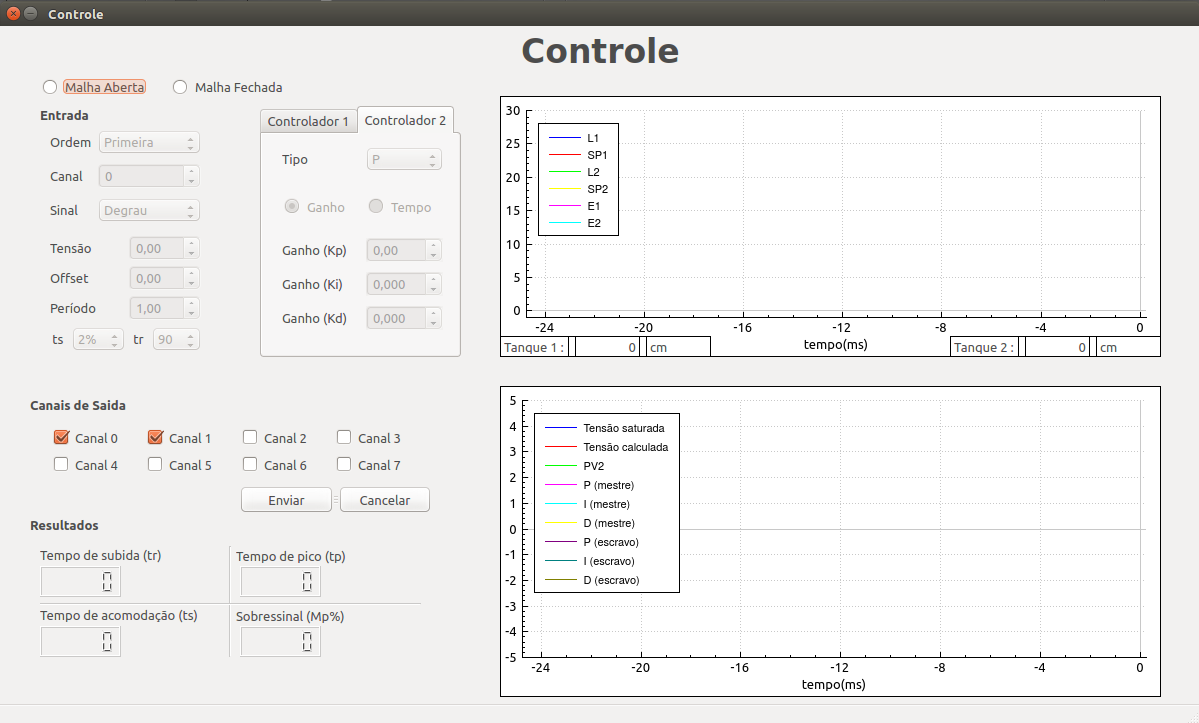
\includegraphics[width=11cm]{ImagensLab4/interface-versao4.png}
\caption{Interface do software de controle}
\label{interface}
\end{figure}

...

%\end{flushleft}

\newpage

%%%%%%%%%% REFERENCIAL TEÓRICO %%%%%%%

\thispagestyle{main}

\section{REFERENCIAL TEÓRICO}

\subsection{CONTROLE EM CASCATA}
\hspace{4ex}O controle em cascata é uma estratégia de controle que utiliza dois controladores aninhados de modo que a identificação de pequenos distúrbios aconteça de forma mais rápida e, consequentemente, a correção seja feita antes de o sistema sofrer grandes alterações. De forma genérica, o controle em cascata pode ser representando pelo diagrama da figura \ref{cascata}. Pode-se perceber que é necessário medir duas variáveis de processos, o da malha interna (chamada de malha escrava) e o da malha externa (chamada de malha mestre). Essas medidas, feitas através de uso de sensores, é comparada com a referência de cada malha. Sendo que a referência da malha externa, ou set point, é uma entrada do sistema. Já na malha interna, quem determina qual vai ser o "nível" a ser alcaçado é o controlador da malha externa. Então a malha do processo secundário recebe o erro, é feito o cálculo do nível para aquele processo que é enviado através de uma sinal de controle para o atuador, modificando o processo da malha interna.     

\begin{figure}[h]
\centering
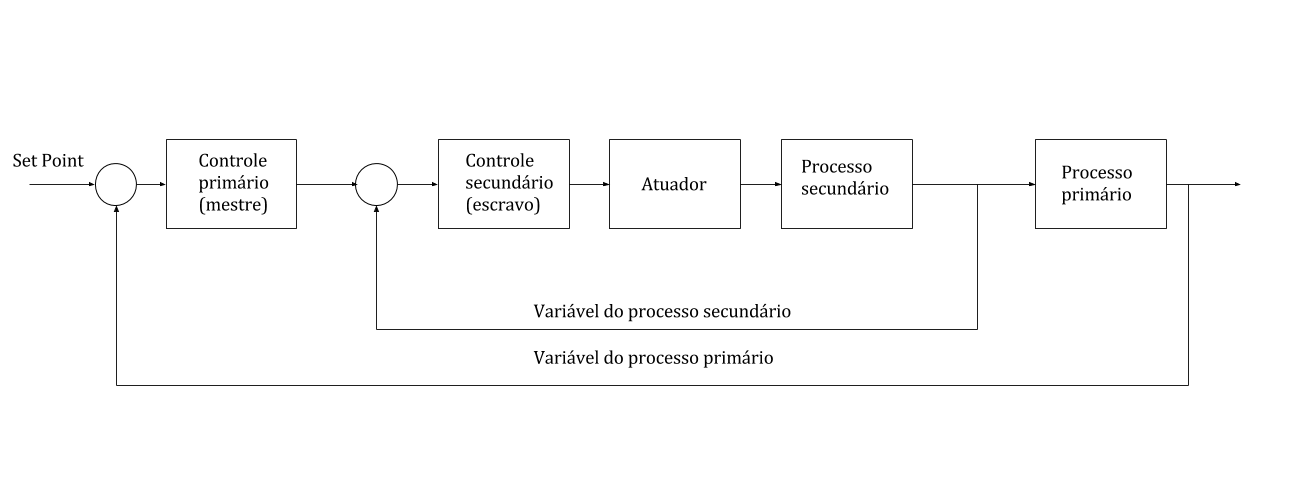
\includegraphics[width=17cm]{ImagensLab4/controle-em-cascata.png}
\caption{Diagrama de bloco do controle em cascata}
\label{cascata}
\end{figure}

Esse tipo de configuração é eficiente devido a dependência entre o processo primário e o secundário. Por exemplo, numa planta onde o gás que passa por um cano é resposável pelo aquecimento da água de um tanque, a atuação é feita controlando a quantidade de vazão do gás no cano. Há uma relação nesse processo em que quanto maior a vazão, mais quente ficará a água. Então a malha mestre seria o tanque com a água, e a malha escrava, a tubulação com gás. 

Outro aspecto importante a ser levado em consideração é a velocidade de cada processo. O processo primário tem que ser mais lento que o processo secundário. Como a temperatura varia de forma mais lenta que a vazão de um gás por uma tubulação, então não haveria conflito entre os sinais de controle. 

A questão de utilizar dois controladores vem dessa diferença de velocidades entre os processos, visto que uma diferença pequena de temperatura geraria um pequeno sinal de erro, logo, se tivesse apenas um controlador, o sinal enviado para controlar a vazão seria pequeno, o que não surtiria muito efeito na temperatura, quase não alteraria ou demoraria muito tempo. Já dois controladores conseguem mapear a relaçao entre o processo lento e um processo mais rápido. 

Uma das desvantagens de se utilizar o controle em cascata é que, ao adicionar mais um controlador, aumenta a complexidade de controle, pois é necessário sintonizar um quantidade dobrada de ganhos, gerando uma quantidade maior de combinações entre tipos de controle e ganhos possíveis. 




\newpage

%%%%%%%%%% METODOLOGIA %%%%%%%%%%%%%%%

\thispagestyle{main}

\section{METODOLOGIA}

\hspace{4ex}Utilizando o simulador R2D2E, foram feitos testes com o controlador mestre e o escravo, como também, com apenas um controlador para alcançar determinados níveis dos tanques da planta, os quais serão expostos nos resultados.

\hspace{4ex}Para isso, foi implementado uma classe controlador a qual é determinada de acordo com as escolhas do usuário, ou seja, se é P, PI, PD, PID ou PI-D. Por exemplo, se o usuário escolhe o controlador PD, ele fornecerá apenas os valores de Kp e Kd, ou Kp e $\tau_d$, e a partir desses valores a classe assumirá que Ki ou $\tau_i$ não existe, ou seja, o valor da integral será zero. O mesmo acontece se for escolhido o PI, nesse caso, o valor da derivada do erro será zero.

\hspace{4ex}Observe os métodos abaixo, o primeiro é para os casos em que o usuário escolher os controladores P, PI, PD ou PID, enquanto que o segundo método foi criado para o caso em que se quer usar o PI-D, pois utiliza o sinal do processo (y) ao invés de usar o erro.
\begin{lstlisting}
double PID::Controle(double e, double h)//Controladores P, PI, PD e PID
{
    I= I+Ki*e*h; //Simpsons (e+e_ant)*h/2 - integral do erro
    D= Kd*(e-e_ant)/h; //Derivada do erro
    e_ant= e; //Erro
    return Kp*e+I+D; //Sinal de controle
}

double PID::Controle(double e, double y, double h)//Controlador PI-D
{
    I= I+Ki*e*h; //Integral do erro
    D= Kd*(y-e_ant)/h; //Derivada do sinal do processo
    e_ant= y; //Sinal do processo
    return Kp*e+I+D; //Sinal de controle
}
\end{lstlisting}
\hspace{4ex}No software desenvolvido, esses valores podem ser escolhidos como mostrado na figura \ref{controladores}.

\begin{figure}[H]
     \centering
     \subfloat[][Controlador Mestre]{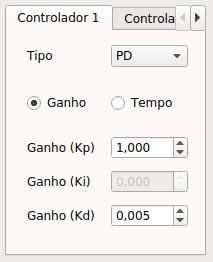
\includegraphics[width=4cm]{ImagensLab4/controlador1}\label{<figureP1>}}\hspace{4ex}
     \subfloat[][Controlador Escravo]{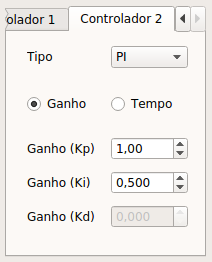
\includegraphics[width=4cm]{ImagensLab4/controlador2}\label{<figureP2>}}\\
     \caption{Interface para a escolha dos controladores}
     \label{fig:controladores}
\end{figure}


\newpage

%%%%%%%%%% RESULTADOS %%%%%%%%%%%%%%%

\thispagestyle{main}

\section{RESULTADOS}
\hspace{4ex}Analisando o observador de estados para varios polos. Onde a curva em azul indica o nivel do tanque 1, a curva em verde o nivel do tanque 2 a cruva em preto o nivel observado do tanque 1 e a curva em cinza o nivel observado do tanque 2.

\hspace{4ex} Inicialmente colocando dois polos em 0, podemos ver que a curva do nivel do tanque 2 ficou em cima da curva original indicando que seus valores estão muito proximos. Já no tanque 1 podemos ver que o valor estimado do nivel se aproxima do valor real mas como o observador está muito rapido, devido aos polos na origem, acaba passando do seu valor.
\begin{figure}[!h]
\centering
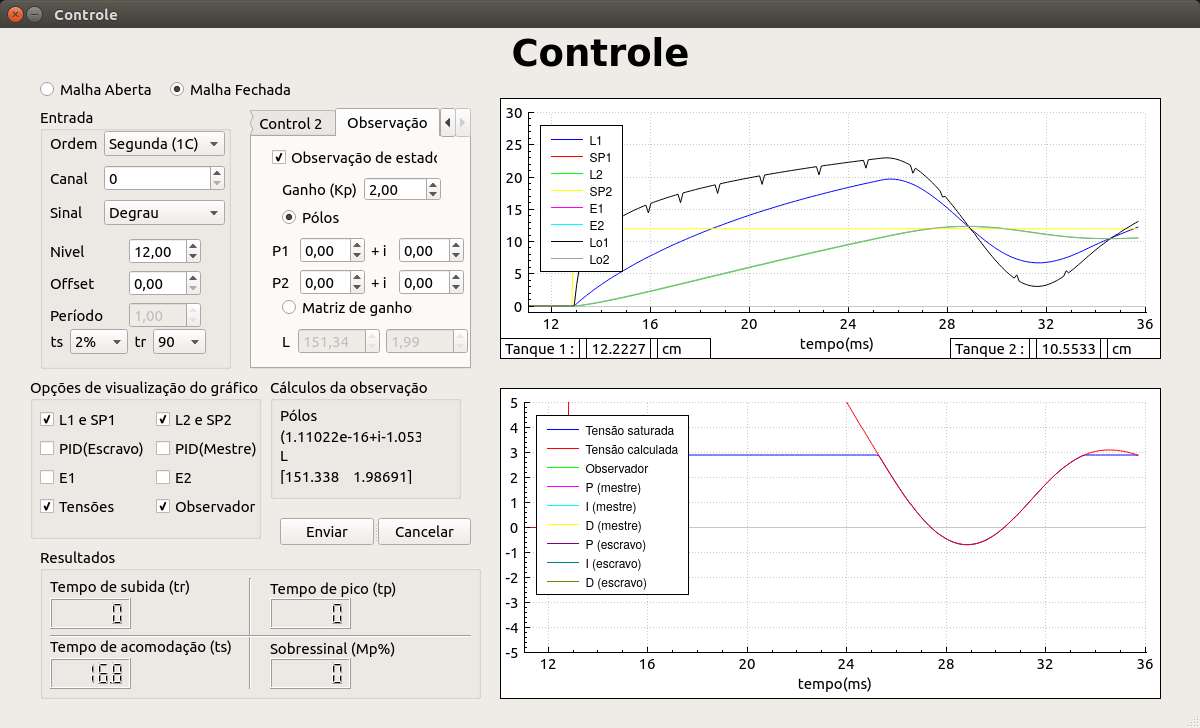
\includegraphics[width=14cm]{FotosObservador/PolosEm01}
\caption{Observador com dois polos em 0}
\label{img1}
\end{figure}
\begin{figure}[!h]
\centering
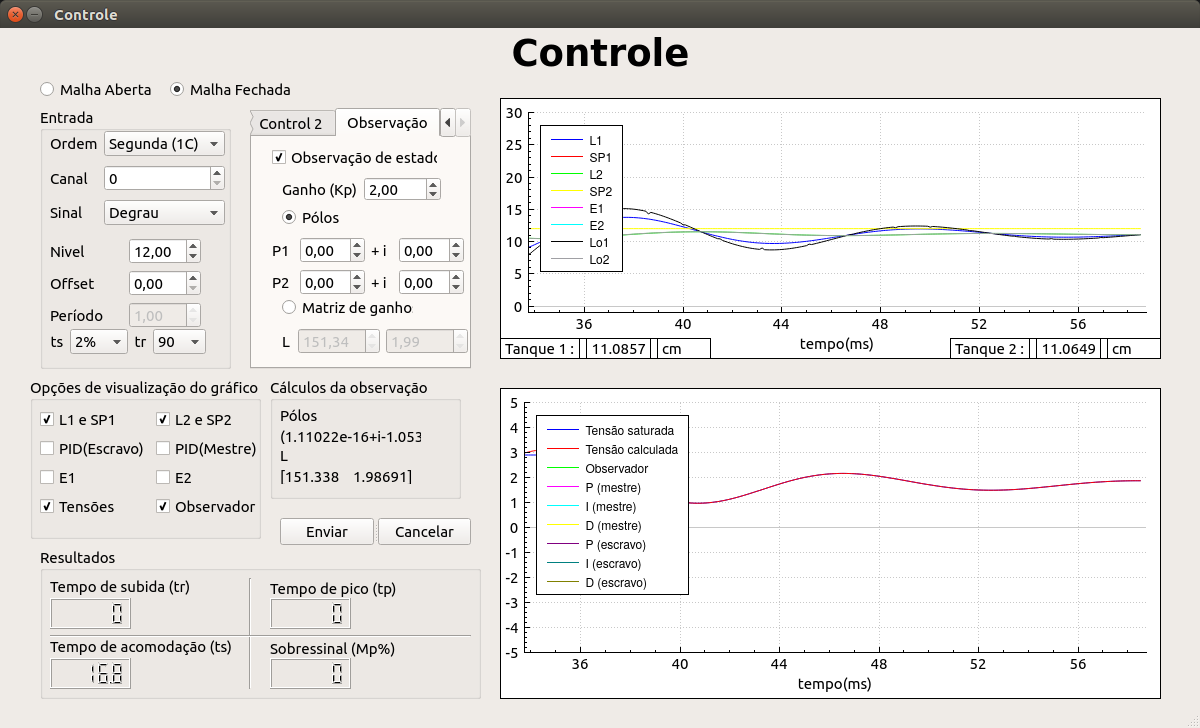
\includegraphics[width=14cm]{FotosObservador/PolosEm02}
\caption{Observador com dois polos em 0}
\label{img2}
\end{figure}

\hspace{4ex} Agora com polos imaginarios em 0.7+0.7i e 0.7-0.7i. O valor observado do tanque 1 foi bastante oscilatorio como esperado e o valor do tanque 2 continuo acompanhando a curva.
\begin{figure}[!h]
\centering
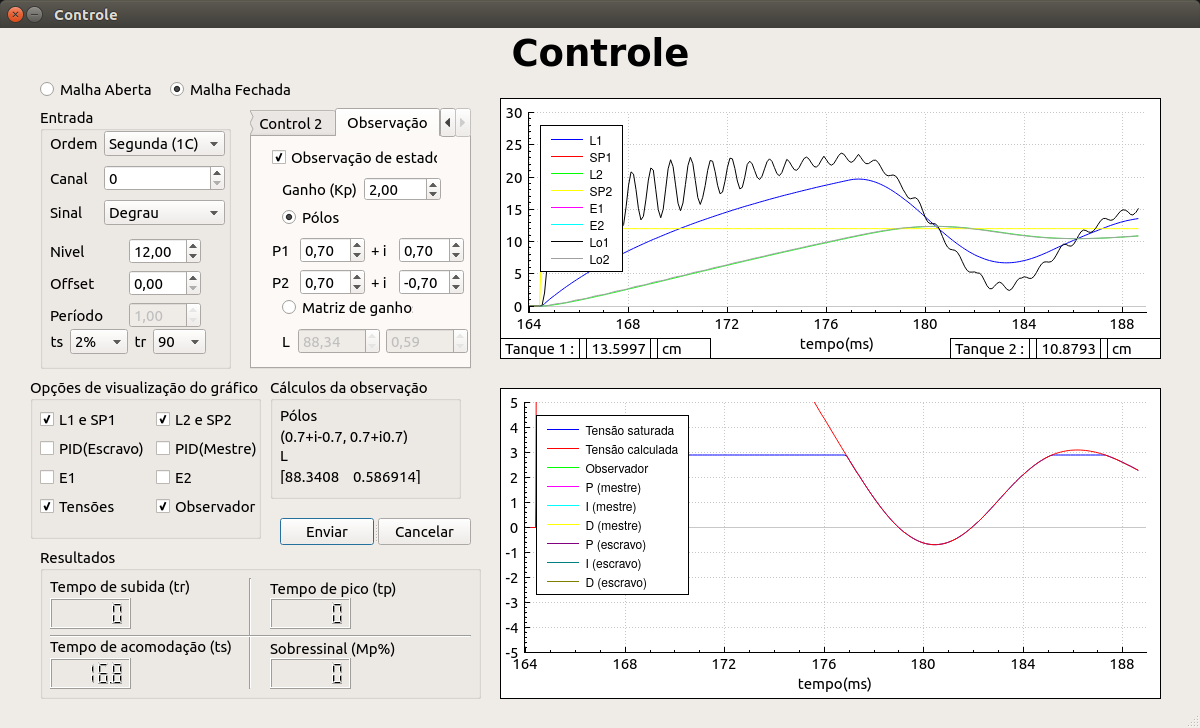
\includegraphics[width=14cm]{FotosObservador/PoloImaginario2}
\caption{Observador com polos imaginarios}
\label{img3}
\end{figure}
\begin{figure}[!h]
\centering
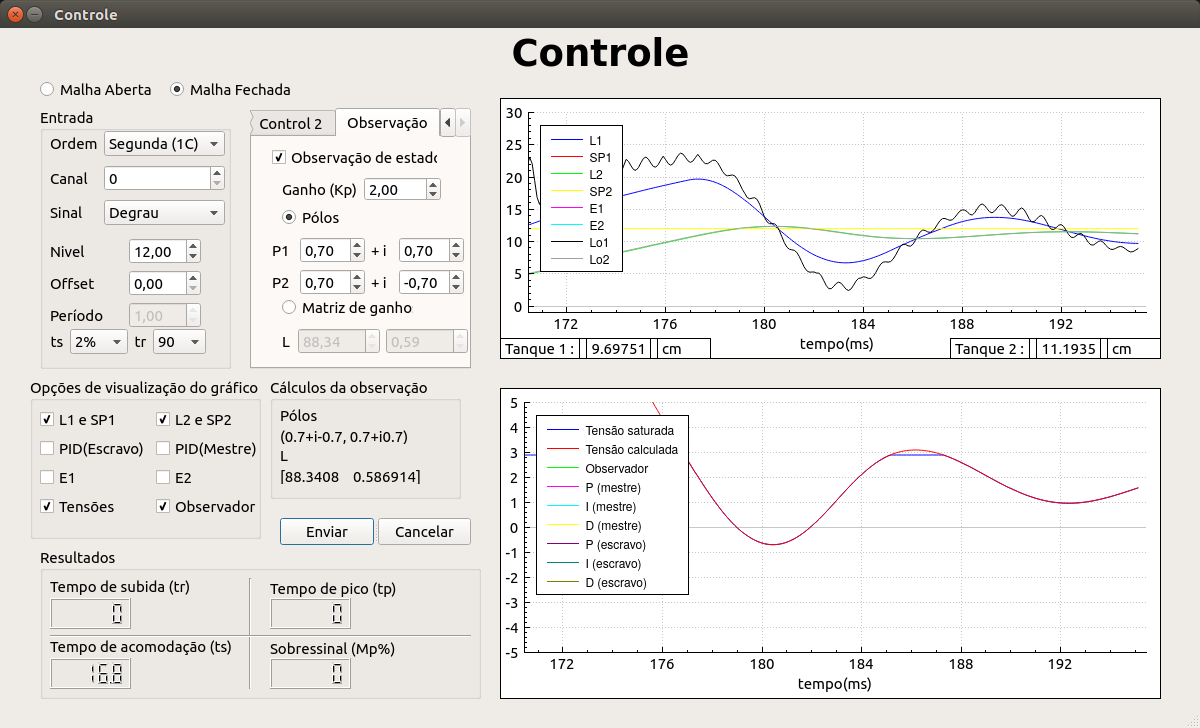
\includegraphics[width=14cm]{FotosObservador/PoloImaginario1}
\caption{Observador com polos imaginarios}
\label{img4}
\end{figure}

\newpage
\hspace{4ex} Agora  com dois polos reais distantes do centro da circuferencia em 0.99 e 0.99, podemos ver que até mesmo o nivel do tanque 2 demora para acompanhar o valor real da curva.
\begin{figure}[!h]
\centering
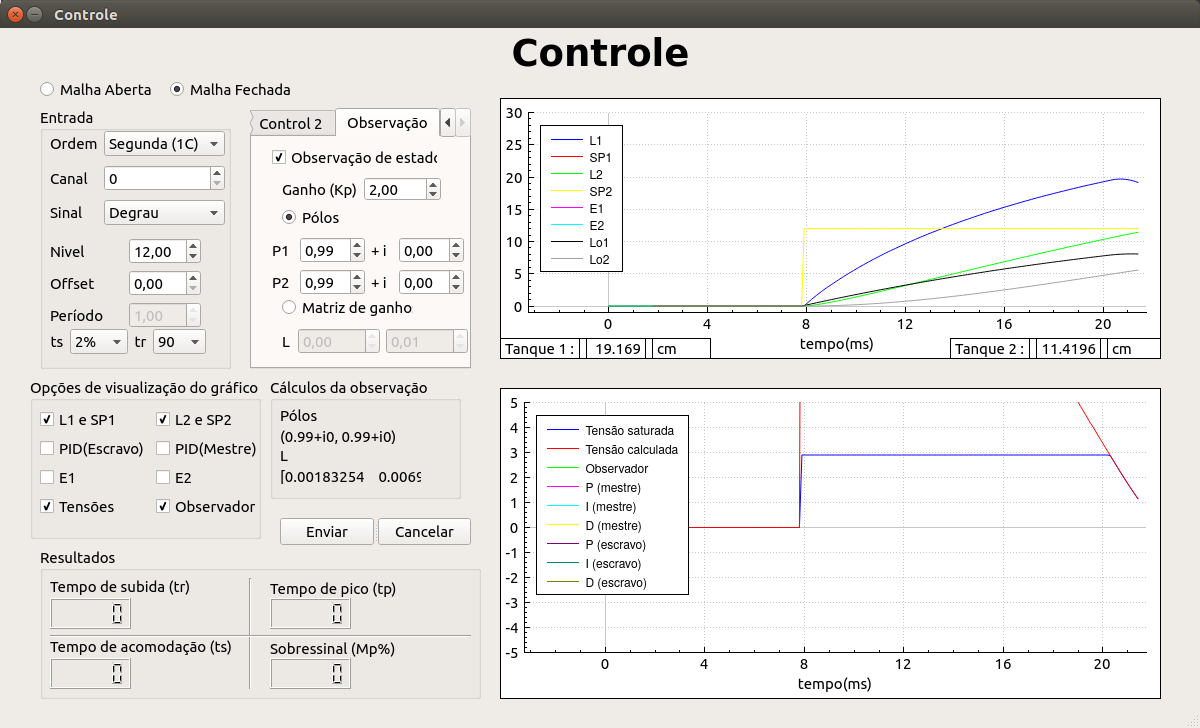
\includegraphics[width=14cm]{FotosObservador/PolosMuitoLentos1}
\caption{Observador com polos distantes da origem}
\label{img5}
\end{figure}
\begin{figure}[!h]
\centering
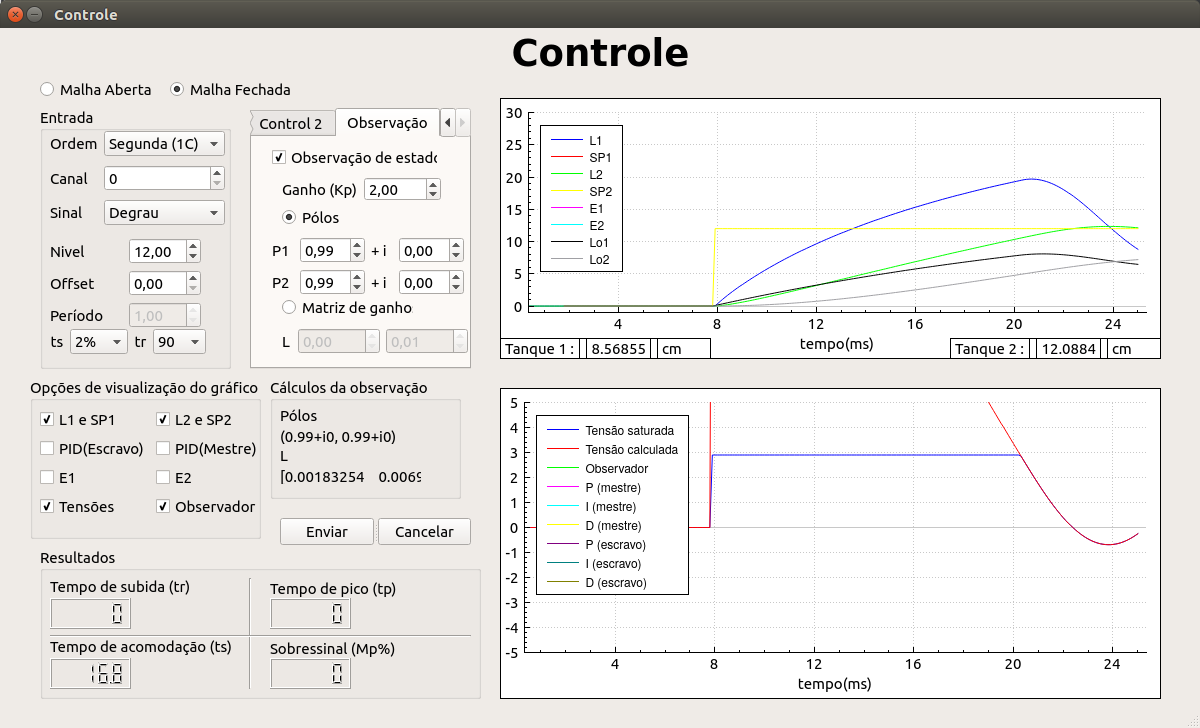
\includegraphics[width=14cm]{FotosObservador/PolosMuitoLentos2}
\caption{Observador com polos distantes da origem}
\label{img6}
\end{figure}

\newpage
\hspace{4ex} Agora com polos reais um na origem e outro distante da origem em 0.99, nessa configuração ambos os valores estimados foram bons.
\begin{figure}[!h]
\centering
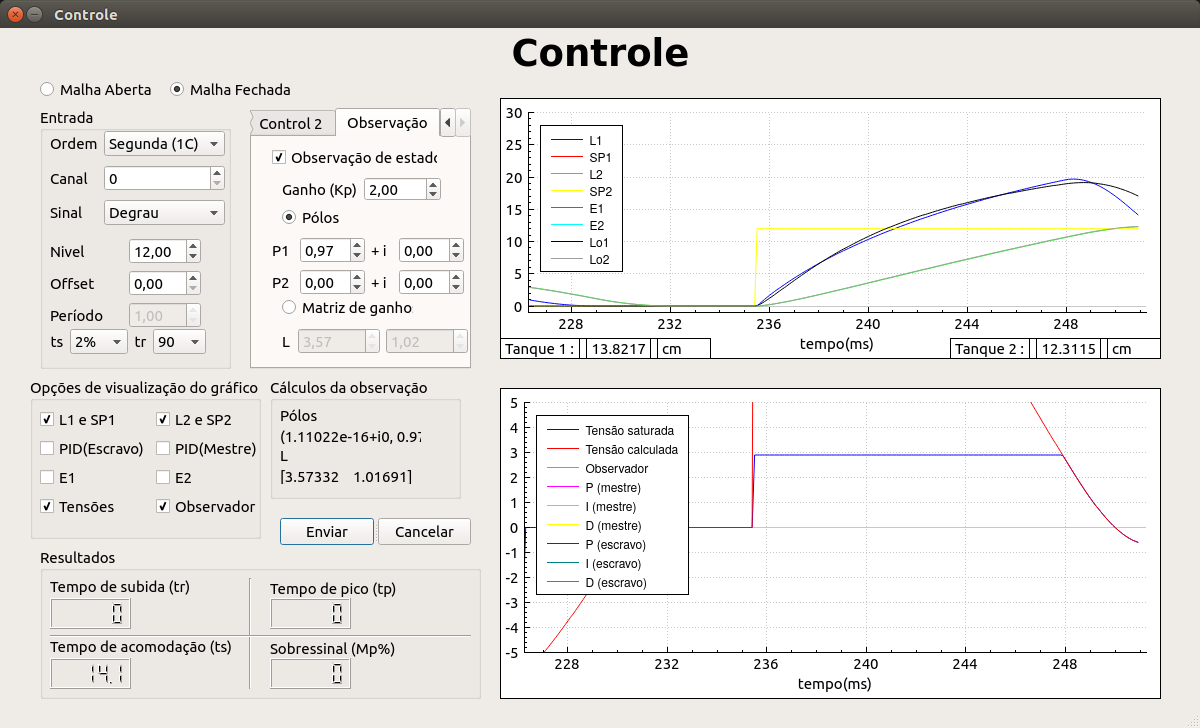
\includegraphics[width=14cm]{FotosObservador/PoloRapidoELento2}
\caption{Observador com um polo na origem e outro distante}
\label{img7}
\end{figure}
\begin{figure}[!h]
\centering
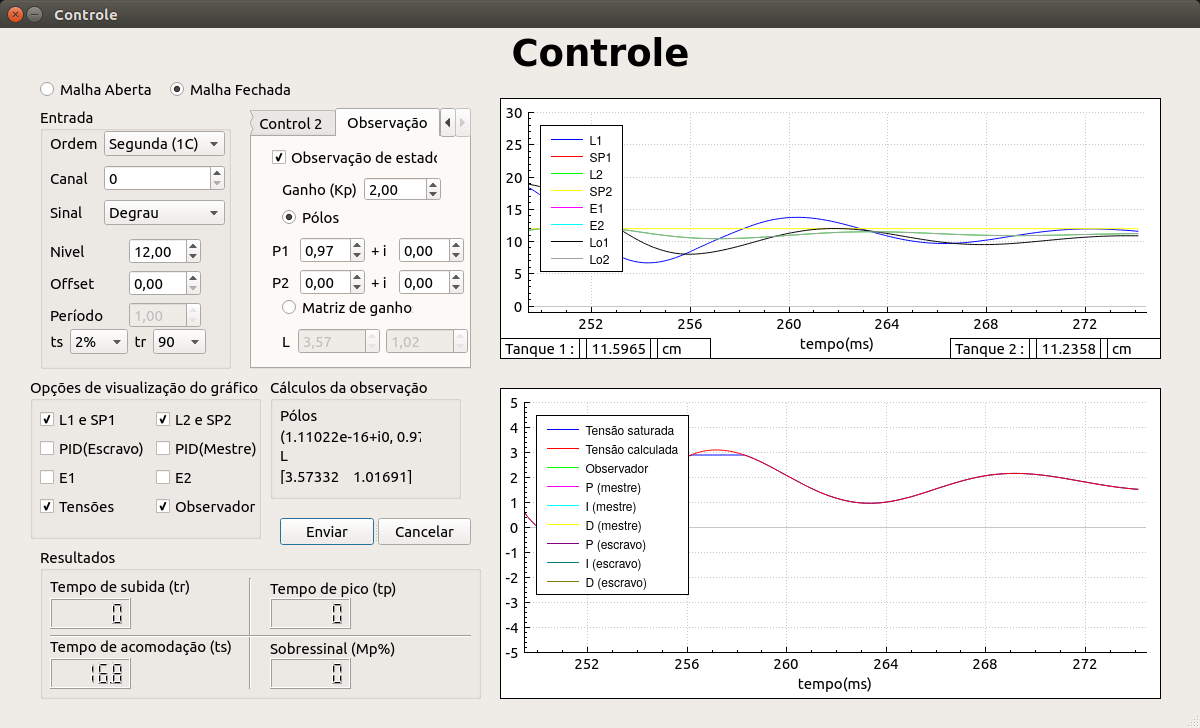
\includegraphics[width=14cm]{FotosObservador/PoloRapidoELento1}
\caption{Observador com um polo na origem e outro distante}
\label{img8}
\end{figure}

\newpage

%%%%%%%%%% CONCLUSÃO %%%%%%%%%%%%%%%

\thispagestyle{main}

\section{CONCLUSÃO}

\hspace{4ex}Os testes realizados mostram que ao utilizar um controlador em cascata aumenta a estabilidade do sistema diminuindo a sua oscilação do tanque 1 e melhorandado o resultado em geral, mas aumenta a complexidade do projeto pois é necessario sintonizar dois controladores.

\newpage
%%%%%%%% REFERÊNCIAS %%%%%%%%%%%%%%%%%

\thispagestyle{empty}
\section{BIBLIOGRAFIA}

Fundamentals of cascade control | Control Engineering. Disponível em: <http://www.controleng.com/single-article/fundamentals-of-cascade-control/bcedad6518aec409f583ba6bc9b72854.html>. Acesso em: 10 maio. 2017.




%Referências bibliogáficas (geradas automaticamente)

%\addcontentsline{toc}{chapter}{Referências bibliográficas}
%\bibliography{bib/bibliografia}

%\appendix

%Apêndice A
%\include{apendice}

\end{document}
